\newpage
\section {Билет 8. Одно-, двух- и трехзвенные архитектуры.}

Основная архитектура приложения может принимать различные формы. Основные различия между архитектурами приложений состоят в количестве систем, участвующих в работе приложения. Эта классификация производится по количеству \textbf{звеньев (tiers)}.

Каждое приложение базы данных состоит из трех отдельных компонент:
\begin{enumerate}
	\item[\textbullet] Службы базы данных (database services). Это конечный сервер базы данных и данные, которые размещены в этой базе данных.
	\item[\textbullet] Службы приложения (application services). Это механизмы манипулирования данными, извлекаемыми из базы данных. Логика их работы определяется приложением или потребностями бизнеса.
	\item[\textbullet] Службы представления (presentation services). Это пользовательский интерфейс. Службы представления должны быть способными манипулировать данными таким образом, чтобы это было понятно пользователям.
\end{enumerate}

\begin{figure}[h]
	\centering
	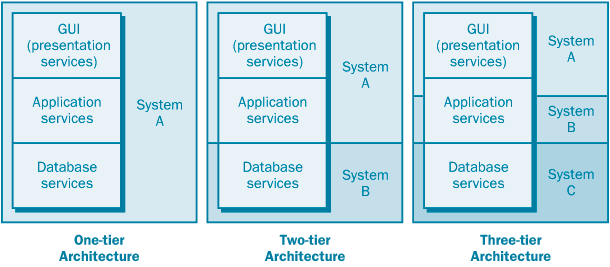
\includegraphics[scale=0.75]{8/08_01.png}
	\caption{Одно-, двух- и трехзвенные архитектуры}
\end{figure}

Различие между однозвенной, двухзвенной и трехзвенной архитектурами зависит от того, каким образом разделяются на части эти компоненты. В однозвенной архитектуре они все являются частями одной программы. В двухзвенной архитектуре эти компоненты разделены на две отдельные части. В трехзвенной архитектуре компоненты разделены на три отдельные части.

Однозвенная архитектура – это система, в которой все службы базы данных, приложения и представления (пользовательский интерфейс) размещены на одной системе. Системы такого типа не производят обработку вне тех компьютеров, на которых они исполняются. Примером однозвенной архитектуры может служить база данных Microsoft Аccess с локальными службами представления.

\bigskip
В двухзвенных архитектурах службы представления и база данных размещаются на разных системах (компьютерах). Уровень служб представления (пользовательский интерфейс) обычно включает в себя логику работы приложения. Хорошим примером двухуровневого приложения является приложение, использующее SQL Server Enterprise Manager. У таких приложений пользовательский интерфейс и логика работы приложения размещаются в Enterprise Manager, но все данные, необходимые для функционирования приложения, находятся в базе данных SQL Server на другом компьютере.

\bigskip
В трехзвенных архитектурах уровень базы данных, уровень приложения и уровень служб представления выделены в три разные компоненты. В типичных трехзвенных приложениях используется промежуточный уровень для обслуживания многочисленных соединений от уровня служб представления, благодаря чему уменьшается количество соединений с SQL Server. Кроме того, этот промежуточный уровень может выполнять значительный объем работы, связанной с реализацией специфики целевых задач (логики предметной области), освобождая базу данных для решения тех задач, которые она выполняет лучше всего, – для доставки требуемых данных.

\bigskip
Фактически, обычно системы начинаются с одного сервера базы данных, соединенного с несколькими серверами приложений, которые, в свою очередь, обслуживают много компьютеров-клиентов. Решения, принимаемые при проектировании системы, зависят от количества ее пользователей и выбранного вами приложения.
